\documentclass[10pt,a4paper]{report}
\usepackage[utf8]{inputenc}
\usepackage[english]{babel}
\usepackage{amsmath}
\usepackage{amsfonts}
\usepackage{amssymb}
\usepackage{wrapfig}
\usepackage{graphicx}
\graphicspath{{./Images/}}
\usepackage{listings}
\usepackage{color}

\definecolor{dkgreen}{rgb}{0,0.6,0}
\definecolor{gray}{rgb}{0.5,0.5,0.5}
\definecolor{mauve}{rgb}{0.58,0,0.82}

\lstset{frame=tb,
  language=Python,
  aboveskip=3mm,
  belowskip=3mm,
  showstringspaces=false,
  columns=flexible,
  basicstyle={\small\ttfamily},
  numbers=none,
  numberstyle=\tiny\color{gray},
  keywordstyle=\color{blue},
  commentstyle=\color{dkgreen},
  stringstyle=\color{mauve},
  breaklines=true,
  breakatwhitespace=true,
  tabsize=3
}
\pagenumbering{roman}

\title{Using Keystroke Dynamics to Authenticate a User Based on their Typing}
\author{Jack Francis}
\date{\today}

\begin{document}

\maketitle

\begin{abstract}
Hello
\end{abstract}

\tableofcontents

\pagenumbering{arabic}

\chapter{Introduction}
\setcounter{page}{1}

\chapter{Survey of Literature}

\chapter{Design and Implementation}

The following procedure from section 3.2 onwards is a rough implementation of the validation procedure by Ramin Toosi and Mohammad Ali Akhaee in their excellent paper 'Time–frequency analysis of keystroke dynamics for user authentication'. \cite{ToosiRamin2021Taok} The paper is theoretical in nature and describes an approach for performing validation on one word and then comparing them. It is in essence a one-time system whilst mine is a continuous system that aims to keep the user safe. In my project I've modified and implemented their validation approach whilst adding data gathering, word forming, word selection, word storage and update function. 

\section{Data gathering and Forming}
My program relies on capturing the users keystrokes and then processing them and then comparing them using a similarity measure. In order to do this, I decided to use the Keyboard Library REFERENCE HERE as it is a lightweight, secure and modern library that makes capturing keystrokes easy. In my project, I make use of the hook function of the library which is used to "hook" onto a users keyboard and record all of the users actions in and create keyboard events for each action. The record function which makes use of this hook function is shown in figure \ref{fig:Record}. The code snippet is very simple, first the program will 'hook' onto the keyboard using the Keyboard Libary mentioned above, record all keystrokes until the interval has passed and then stop recording. The start time of the interval and an array of Keyboard Events are then returned to the main body of the program. The start time of the interval is recorded and returned as it used further on in order to be able to place keyboard events on a time line in the context of the interval.

\begin{figure}[h!]
	\begin{lstlisting}
		def record(interval):
    		recorded = []
    		startTime = time.time()
    		keyBoardHook = keyboard.hook(recorded.append)
    		time.sleep(interval)
    		keyboard.unhook(keyBoardHook)
    		return recorded, startTime
	\end{lstlisting}
	\caption{Record Function}
	\label{fig:Record}
\end{figure}

A keyboard event is generated every time the user does something on the keyboard, whether that be pressing or releasing a key. Further information such as the type of the action (whether it was an a press or a release), which key is this action happening on and a a highly accurate time stamp of when the event occurred. Figure \ref{fig:Hook}, shows an example of a keyboard event produced by the function when the user presses down the 'h' key.

\begin{figure}[h]
\centering
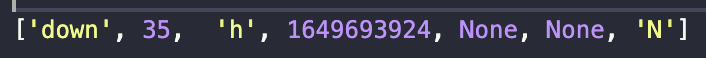
\includegraphics[scale=0.97]{KeyboardEvent}
\caption{The keyboard representation of a user pressing "h"}
\label{fig:Hook}
\end{figure}

The first element in the array is the action, this can be either 'up' or 'down' which are both self-explanatory. The next field is the scan-code which is a field I don't use but is useful for identifying keys easily. After this, is the name of the key which in this case is 'h' as we pressed the 'h' key down. The next field is the time since the epoch in seconds which is useful as it is this precise time-stamp that is used to do the rest of the calculations. The other three fields are device, modifiers and whether or not the user used a keypad. None of these I use in my program and as such are discarded almost immediately.

A small amount of pre-processing is then done on this data before it is paired up. The first step is to remove the scan code, keypad, modifier and device from each keyboard event and convert them into something lighter and more usable. The next step is to take the start time that is returned by the record function and subtract this from the time stamp in each keyboard event to get the time that the action occurred in the interval. Figure \ref{fig:preproc} shows what the data in \ref{fig:Hook} looks like after going through this.

\begin{wrapfigure}{l}{0.5\textwidth}
	\begin{center}
		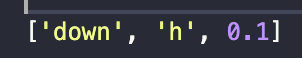
\includegraphics[width=0.48\textwidth]{KeyboardEventPreProc}
	\end{center}
	\caption{Keyboard representation of a user pressing 'h' after pre-processing}
	\label{fig:preproc}
\end{wrapfigure}

The data collected at this point is stored as a 2D array with each sub array corresponding to an action. An example sub array is shown in \ref{fig:preproc}.

In this form the data is unable to be used for anything, as it currently takes the form of a number of individual actions seem to have no relation to one another. Therefore, the next step is to form pairs from the data. A pair is formed of when 'down' action and one 'up' action where the key field matches and the 'down' is before the 'up'. The reason this is done is that it allows the program to work half as much data which reduces the number of unnecessary data points and allow the program to be able to form words using these pairs.

\begin{wrapfigure}{r}{0.4\textwidth}
	\begin{center}
		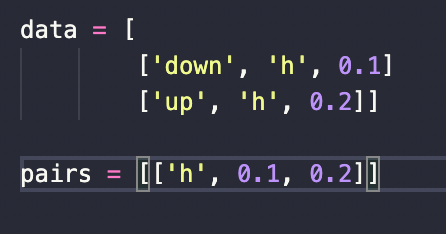
\includegraphics[width=0.38\textwidth]{SimplePairing}
	\end{center}
	\caption{Example of simple pairing}
	\label{fig:SimpPair}
\end{wrapfigure}

There are two main rules to follow when pairing the data. Due to the nature of how the data is collected, it is currently stored in chronological order which is very useful. In many cases, the user will press and release a key in quick succession without pressing any other keys. Due to the chronological nature of the data, pairing theses types of presses is easy. All that is needs to be done is to iterate through the pairs and when we come to a 'down' action then simply select the next value in the array if it is an 'up' action and the key matches. Figure \ref{fig:SimpPair} shows an example of this type or pairing. However, this type of nice easy matching is not always the case.

In some cases, a user may press more than one key down at once. This might occur when the user is capitalising words using 'shift' or when the user is typing fast so they may be already pressing down the next key before releasing the previous. An example of what the data will look like when this is the case is shown in Figure \ref{fig:WrongPair}. Applying the previous method in which we pair up keys with matching key types and opposite actions which are next to each other would result in the output shown in the pairs array. As you can see, this is not correct and would only lead to one pair where there should be two.

\begin{wrapfigure}{r}{0.4\textwidth}
	\begin{center}
		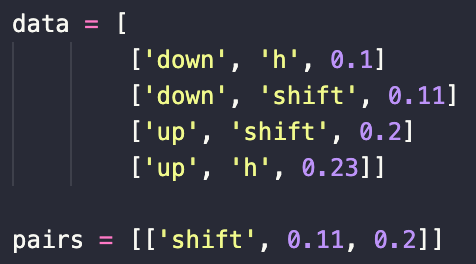
\includegraphics[width=0.38\textwidth]{PairingWrong}
	\end{center}
	\caption{Example of simple pairing}
	\label{fig:WrongPair}
\end{wrapfigure}

In order to fix this, it is necessary to include another case in the code. If the current action doesn't have a matching key and opposite action next in the array, then the program will iterate through the rest of the array starting from the current point in it searching for the next entry with a matching key and an opposite action that is after the current. If it finds one it will then pair them up. The key thing we assume for this to work is that every action has an opposite action. In nearly all cases we assume this to be true as it is highly unlikely that a user will hold down a key for the entire interval. If in a rare case this occurs however, this is handled. If the method cannot find a pair, then it is still added to the pairs list with an end time of the length of the interval.

The finished algorithm is shown in Figure \ref{fig:PairForm}. The reason for the error handling is that when coming to the end of the data, attempting to access the next element to check if it can be paired up results in an index error.
\begin{figure}[h!]
	\begin{lstlisting}
		def rawPairs(self):
        """
        Converts the array from the process function into key pairs

        Returns:
            2D array: Consisting of a pair of actions from the array above.
        """
        pairsArray = []
        for i in range(len(self.processed)):
            try:
                
                if (self.processed[i][2] == 'down' and self.processed[i+1][2] == 'up' and self.processed[i][0].lower() == self.processed[i+1][0].lower()):
                    # If the next value in the array is the up action
                    pairsArray.append([self.processed[i][0], self.processed[i][1], self.processed[i+1][1]])
                else:
                    # Otherwise, search for the next opposing action and pair them up
                    for x in range(i, len(self.processed)):
                        if (self.processed[x][0].lower() == self.processed[i][0].lower() and self.processed[x][2] == 'up' and self.processed[i][2] == 'down'):
                            pairsArray.append([self.processed[i][0], self.processed[i][1], self.processed[x][1]])
                            break        
            except IndexError:
                pass
        return pairsArray
	\end{lstlisting}
	\caption{Pair Forming Function}
	\label{fig:PairForm}
\end{figure}

The resulting pairing algorithm shown in figure \ref{fig:PairForm} has a time complexity of \(O(n^2)\). In a program which is all about speed and minimal impact to the user, it is essential that the program has a the lowest time complexity as possible. Due to the complicated nature of how users type I believe this is the best time complexity for a problem of this nature.

\subsection{Forming Words}

After forming the pairs, the next step is to form words from these pairs. The words that the program forms are essential as it is this that the program uses to compare users. In English words take many forms, as such it is needed to account for many different possibilities in the word forming function. This function takes in the list of pairs and returns an array of word objects. The reason I decide to pivot to an object orientated approach at this point in time is that these words are heavily utilised and I would like to have methods attached to them. For example, it is far easier to generate the Key Down Signal mentioned in following sections on a word by word basis rather than having one function in the main body of the calculation class. This reduces the amount of lines written and makes code easier to read and understand.

A word is defined in my program as a sequence of pairs bounded by punctuation, white space or the use of modifiers such as 'shift'. In latter stages of this report, I refer to these as break pairs. The one notable exception to this rule is when an apostrophe or a hyphen is detected. If this occurs, then the program will check the previous pair and the pair afterwords and if both are letters and not numeric or punctuation, the the pair is added to the word. 

The data at this stage takes the form of a 2D array. The program will iterate through the 2D array it is given and check the key that the pair matches. If it is a letter or a number then it is added to another array which is used to store the current word being formed. If a break pair is found, it is not added to the current word, the current word is used to form a word object which is then saved to an output array and in some cases further action will be taken depending on what type the break pair takes. If the break pair is a white space pair then the pair is simply skipped.. However, if the break pair is a modifier such as 'shift' or 'ctrl' then the relevant entry in the semantics dictionary is updated for that user. This dictionary is used in the validation section of the project and is another indicator on how a user types. Backspace handling is done separately. If the user has pressed backspace, then the last letter added to the word is removed from it. The program can handle multiple backspaces even if they delete the entirety of the current word. If this occurs, the previous word object is popped off the array to be the current word and the last letter of this new current word is removed.

When the program gets to the last pair in the input array, if the pair is not a break pair then the pair is added to the current word and the current word forms a word object which is then saved to the output array.

The program will then return the output array which at this time is formed of word objects and the semantics dictionary. The output array is then saved to the wordsOut attribute of the Calculation class while the semantics is saved to the semantics attribute in the class.

The state of the data after this section is simple. The data is an array of word objects. Each word object is in essence an array of pairs with associated timings attached. This whole section could be defined as the pre-processing of the data to get it into a format that can be used in order to perform similarity calculations.

\subsection{Data Selection}

If the program was to go through and check every single word for similarities, the cost in terms of time would be excessive and would make the program unfit for use especially if the user typed quickly during the interval. For example, if the program checked every word and the user typed 56 words in a 60 second interval, the time taken would be over 2 minutes as shown in figure \ref{fig:WordsvsTime} which while highly accurate and secure would render the program unusable as the time taken to process and perform all the similarity calculations would be in excess of the interval and as such would lead to a lower degree of accuracy and security. Furthermore, this would severely impact the performance of the users computer and as such go against one of the main aims of the project.

As such, it is necessary to use a sampling method to choose words from the list of words chosen by the word forming function. While this is less accurate than checking every word, the performance gain over checking every word is huge with on average time saving of XX per interval. Choosing how many words were selected was the next problem I endeavoured to fix.

I conducted a number of tests measuring how long the entire validation procedure took. Initially I started with 2 words chosen per interval with one chosen every at the start of the interval and one at the end. I then increased the number of words chosen by two each time with the interval remaining the same. At each testing point, the interval remained the same with a word selected using the calculation if figure \ref{fig:Choose} Figure \ref{fig:WordsvsTime} shows the results of such a test. The time taken to perform the calculation increases linearly as the number of words chosen increases. If the, word chosen is particularly long then the time taken increases. The test data was the same for all tests with the user typing a paragraph containing 57 words of differing lengths. Figure The test data along with the raw data collected and the code can be seen in Appendix A. 

\begin{figure}
	\centering
	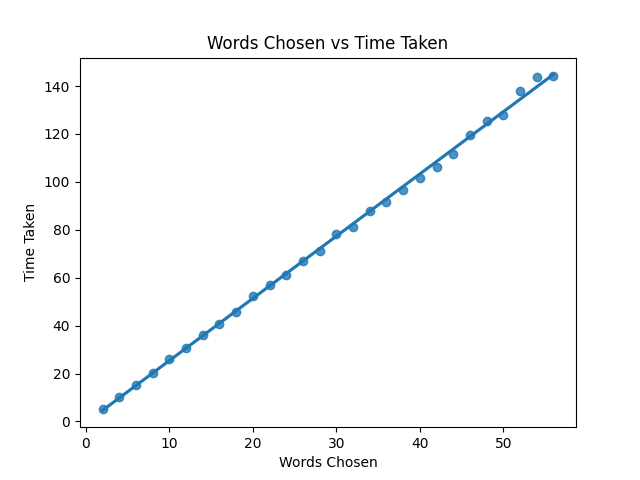
\includegraphics[scale=0.70]{WordsChosenVsTime}
	\caption{Comparing words chosen to time taken in seconds}
	\label{fig:WordsvsTime}
\end{figure}

After performing the test, I settled on the program choosing four words per interval. Choosing four words took under 10 seconds and allowed the program to get coverage every quarter of the interval which is an acceptable level of coverage.

The process to select 4 words from each interval is simple. Given the word list returned by the word former, the program performs the calculation shown in Figure \ref{fig:Choose} where \(w\) is the word list \(n\) is the number of words in the words lists returned by the word former and where \(k\) is the amount of words to be chosen.

\begin{equation}
\textit{EveryX}(w) = \frac{n}{k}
\label{fig:Choose}
\end{equation}

This value returned by this equation is then used in the main body of the function. First of all the program chooses the first value in the words list and adds it to the output. It will select the value returned by figure \ref{fig:Choose}. After doing this, it will add on the value returned by the equation again and select the word at that index again. This will keep happening until either the amount of words selected by the program is the number of words to be chosen. The resulting words are then returned by the function to be used in the rest of the program. 

\section{KD Signal}
Once the raw keystroke data has been formed into words and the words chosen, the next step is to transform the data from a word object made up of keystroke pairs into numerical data that can be used by later algorithms such as Dynamic Time Warping (DTW) and the correlation coefficient. The best way to do this is to transform the data into a measure of how many keys are being held down at a particular point in time. The resulting output is known as a key down signal (KDS). \cite{ToosiRamin2021Taok}

To convert a word into a key down signal, the start and end times of the word being transformed are used. Assume that \(w\) is the array of times that key actions occur in a particular word. \(w_1\) being the time of the first action and \(w_n\) being the time of the last action. This part will loop through all timestamps until it ends with the final time which is denoted by \(w_n\). The accuracy of this step is paramount as it is the level of detail that is the base accuracy for the rest of the steps. A higher accuracy means that the program will check more data points within this range at the cost of reduced performance as the level of points being checked increases. The current level of this is set to 4 decimal points which seems to provide a good balance between accuracy and performance. However this is customisable.
\begin{equation}
\textit{KDS}(w) = \sum^{w_n}_{i=w_1}K(w_i)
\end{equation}
\(K\) is the next step of the algorithm and is heavily based on the KDS algorithm shown in \cite{ToosiRamin2021Taok}. \(n\) is the array of key presses that is used in the previous step. This step of the algorithm iterates through all the key presses and uses a modified Heaviside step function denoted by \(h\) which is run twice per pair with the time input from the previous denoted as \(t\) and the 'down' action denoted as \(n_i^1\) and the 'up' denoted as \(n_i^2\). The value returned by the Heaviside step function with the 'up' action is subtracted from the value returned by the 'down' function.
\begin{equation}
\textit{K}(t) = \sum^{n_k}_{x=1}h(t,n_i^1)-h(t,n_i^2)
\end{equation}
The reason for this subtraction is that the purpose of this measure is to return the number of keys pressed down at the time input. Once a key has been released it is essential that the key is removed from the measure. For example, if a pair exists with down action time being at 1 second and up action time being 1.1 seconds. At time, 1.5 the equation will equal \(1-1=0\). However, if the time put in is 1.05 then the equation will be \(1-0=1\) which indicates that one key was being held down at this particular time.

For every time input, each pair is checked with the sum of all the results stored in a dictionary along with the time input as the key. It's this dictionary that forms the KD signal and is used in further steps.

\subsection{Heaviside Step Function}
This is the bottom layer of the KD signal algorithm. It is a modified version of the Heaviside Step function.
\begin{equation}
	h(x_1, x_2) = \begin{cases}
	1 & \text{ if } x_1 > x_2 \\
	0.5 & \text{ if } x_1 == x_2 \\
	0 & \text{ if } x_1 < x_2
\end{cases}
\end{equation}
The modification done is very simple, the only change is the addition of a third case which tests if the two times are equal to one another. Due to the nature of the use case for my project, there is a relatively high chance that the two times are equal to one another. In this case this means that the user at this time is currently in the process of performing that action whether that be pressing or releasing the key. The

\subsection{Output}
The resulting signal can be shown easily in graph format. fig 1.1 is the KD signal produced by a genuine user whilst fig 1.2 is the signal produced by an imposter user typing the same word.
IMAGE GOES HERE

\section{Dynamic Time Warping}
\subsection{Path}
\subsection{Cost Matrix}
\section{Validation Measures}

Finally the data is in a state where we can perform validation. In order to improve the accuracy of the program, I use two different validation methods along with the semantics collected in the word forming stage. 

The two methods I use along with the semantics are euclidean distance which is done in the dynamic time warping stage. This has secondary importance compared to the 2D correlation co-efficient. The reason for this, is that the euclidean distance is simply a measure of the distance between two points. This is not done on the warped data that is produced by the Dynamic Time Warping which contrasts to the 2D correlation co-efficient. Therefore, I use this as a rough figure and use the correlation co-efficient as the main method. 

The values produced by these validation methods are then put together to form a value between 0 and 100. This is then compared against the confidence interval. The confidence interval is a integer which determines how similar the data loaded in from the file and the data collected in the interval have to be. For example, if the validation methods in the interval (Similarity Score) return a value of 0.75 and the confidence interval is 0.8, then the user is rejected and asked to re-authenticate. Only the euclidean distance and the 2D correlation go into calculate the similarity score. The semantics are used to either raise the confidence interval or lower it depending on the value returned by the semantics validation.

\begin{wrapfigure}{r}{0.4\textwidth}
	\begin{center}
		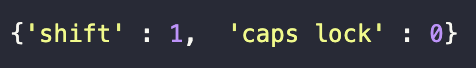
\includegraphics[width=0.38\textwidth]{SemanticsEx}
	\end{center}
	\caption{Example of a users semantics file}
	\label{fig:sem}
\end{wrapfigure}

The semantics validation is very simple. In the words step of the validation procedure, the semantics of the data input is collected and stored in the class. Each user will also have a semantics file stored in their data directory. An example of a users semantics file is shown in figure \ref{fig:sem}. The data stored in the file and the data collected for that interval are then compared against one another. If for example, the user in the past has used the shift key and in this interval has also done so, then the confidence interval is lowered by 0.02. However, if the user in the past has always used the caps lock key and never shift then they don't match and the confidence interval is raised by 0.02. The reason of such a small change in the confidence interval is that users habits regarding this are not typically set in stone and as such any large change will likely lead to reduced accuracy. For example, users will typically use shift when there is a single letter to be capitalised and will use caps lock when capitalising multiple keys. 

The validation methods are explained further in sections 3.4.1 and 3.4.2 respectively. Here I will outline the entire validation process. The flow chart in figure \ref{fig:valProc} provides a visual representation of the first part of the validation procedure. A clearer version is provided in Appendix B.

\begin{wrapfigure}{l}{0.4\textwidth}
	\begin{center}
		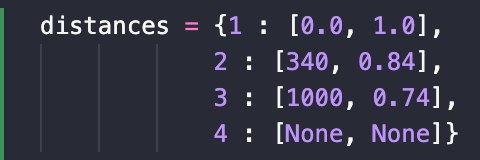
\includegraphics[width=0.38\textwidth]{DistancesDict}
	\end{center}
	\caption{Example of a distances dictionary after validation calculations done}
	\label{fig:distances}
\end{wrapfigure}

As shown in figure \ref{fig:valProc}, the words chosen in the first step are iterated through. If a word already has a word file stored in the users directory then that is loaded in and decompressed. Otherwise, the procedure just returns two None values. The two data sets, one loaded in and the other generated from the current interval are then both put through Dynamic Time Warping where the euclidean distance is calculated and stored. The path generated by the DTW is then used to 'warp' both datasets. It is at this stage that the 2D correlation co-efficient is used in order to calculate one element of the similarity score. The Euclidean distance and the correlation co-efficient are then stored in a dictionary with the key being the index in the chosen array. Figure \ref{fig:distances} showcases an example distances dictionary. In the example, the first two elements were typed by a genuine user with the third being typed by an imposter and the last word has not been seen before so the validation procedures just returned None.

After the distances dictionary has been formed with all values inside. The next step is to categorise the values. First of all we have to define the confidence level for each validation procedure. As shown in the flowchart (\ref{fig:valProc}), these are adjusted based on the results of the semantics validation. The values these take is further discussed in Chapter 4: Results and Discussion. The distances dictionary is iterated through and each value checked. Figure \ref{fig:DistanceTransform} below shows what happens in each individual case where \(e\) is the Euclidean Distance, \(c\) is the value returned by the correlation co-efficient, \(i\) is the confidence level for the correlation co-efficient and \(b\) is the confidence level for the Euclidean Distance.

\begin{equation}
	\begin{cases}
		\textit{None} & e == \textit{None or } c == \textit{None} \\
		\textit{True} & c >= i \textit{ and } e <= b \\
		\textit{True} & c >= i \textit{ and } e >= b \\
		\textit{False} & \textit{Otherwise}
	\end{cases}
	\label{fig:DistanceTransform}
\end{equation}

The value returned by this function is then adding into an array which is used in the next step. Figure \ref{fig:wordCheck} shows what resulting array formed by putting the data in \ref{fig:distances} through this part of the validation procedure. This example presumes that the confidence intervals for Euclidean Distance and correlation co-efficient are 1000 and 0.84 respectively.

\begin{figure}[h]
	\centering
	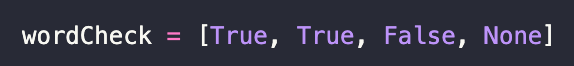
\includegraphics{WordCheck}
	\caption{The result of the data in figure \ref{fig:distances} after going through further validation}
	\label{fig:wordCheck}
\end{figure}

Transforming the data this way allows the order of the data to be preserved. Furthermore, it allows the next stage of the validation to simplified heavily as rather than working with variable data, we know to need to only consider whether the value is one of True, False or None which vastly simplifies the complicated system used to make a decision which is explained in the next step.

The "wordCheck" array shown in \ref{fig:wordCheck} is then used in the next step in order to finally perform an action based on the data. Despite what happens next only three outcome occur. Figure \ref{fig:If1} showcases what happens if only one word is in chosen and an output returned to it. If the word is true, then the person checks out and the program moves on to the next interval. However, if the word doesn't pass the validation checks or has never been seen before, then further processing has to be done. 

This is very complex. If the user fails validation then their pc is locked and they are forced to re-authenticate. At the start of my project, I was planning on creating a separate register and login system however I dismissed due to the fact that users don't want another login system and that the default windows login screen does everything to a greater standard than I ever could. In order to perform this action, I load in the default python library sub process \cite{subprocess} which I then use to call the windows lock dll file. This enables me to lock the user out of the computer easily and efficiently without much wasted code or overhead in terms of performance. If the user has changed when the user does re-authenticate, then 'New' is returned. This tells my main body of the program that it is a new user and as such a new keyboard is created for that user. Keyboards and user storage are explained in \ref{sssec:Storage}. If the opposite happens and the user is re-authenticated successfully, then the word files and semantics are updated and the program returns true.

The validation function can take in as a parameter a 'mode'. This determines what happens should validation fail. The default mode is 'r' which stands for real. This allows the program to do the entire process including locking the users computer if validation fails. 'rnl' stands for real no lock which is mainly used for testing and demonstration purposes because it stops the users pc locking and just returns false. A 't' flag also exists, this indicates that the program is in test mode and when in test mode the program will simply save every word. 

\begin{figure}[h]
	\centering
	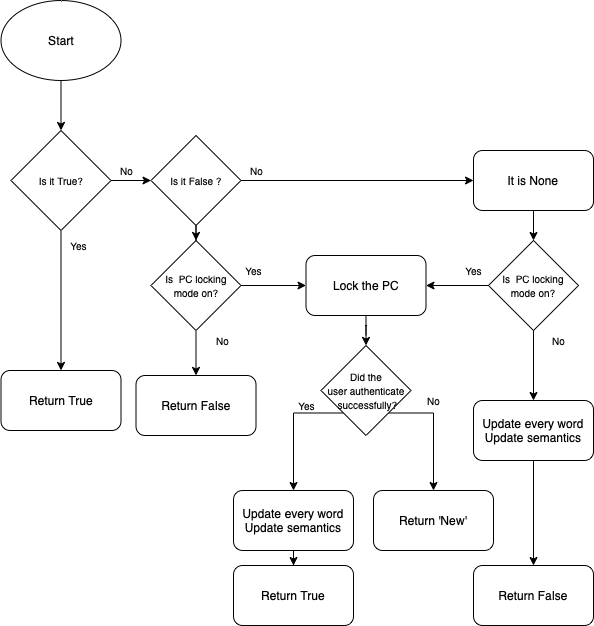
\includegraphics[scale=0.4]{IfLen1}
	\caption{Flowchart which illustrates decision tree if only one word is chosen}
	\label{fig:If1}
\end{figure}

\begin{itemize}
	\item Talk about selecting values
	\item What effect does semantics have?
	\item Weighting of Euclidean vs correlation
	\item Chosen auth method
	\item In all cases what happens?
	\begin{itemize}
		\item If not seen word before
		\item If all validated
		\item If all bar one are validated
		\item etc
	\end{itemize}
\end{itemize}
\subsection{Euclidean Distance}

The first validation method used is the
\subsection{Correlation Coefficient}

\begin{wrapfigure}{l}{0.4\textwidth}
	\begin{center}
		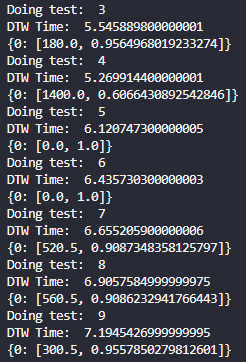
\includegraphics[width=0.38\textwidth]{EucVs2D}
	\end{center}
	\caption{Euclidean Distance compared to 2D correlation co-efficient}
	\label{fig:VCompare}
\end{wrapfigure}

2D correlation co-efficient is used because it is relatively lightweight, quick, easy to implement and provides easy to interpret results. As opposed to the value produced by the euclidean distance, the output returned by the 2D correlation co-efficient can only take a range of values between -1 and 1. If the function returns 1, then the two signals input are exactly the same, 0 if they are radically different and -1 if they are the same again. An example of the output returned can be seen in the second element of the dictionary in figure \ref{fig:distances}. In shortened form, the 2D correlation figure essentially returns a percentage of how close the two input signals are.

This measure is used after the dynamic time warping and take the two input signals as inputs. This is weighted higher in my system due to the stronger accuracy and ease of use. One example of why the this is more accurate than euclidean distance is shown in the figure \ref{fig:VCompare}. 2D correlation co-efficient returns around 0.95 for both, whist euclidean distance returns 180 and 300 which are wildly differing figures.
\begin{equation}
	f(a,b) = \frac{\Sigma^n_{i=1}(a_i-\overline{a})(b_i - \overline{b})}{\sqrt{\Sigma^n_{i=1} (a_i-\overline{a})^2}\sqrt{\Sigma^n_{i=1}(b_i-\overline{b})^2}}
	\label{fig:corrco}
\end{equation}

Figure \ref{fig:corrco} shows the equation that my implementation is based upon where a and b are the two warped arrays passed in, \(n\) is the length of either array, \(a_i\) and \(b_i\) are the values at positions \(i\) in each array respectively. My code implementation is shown in figure \ref{fig:CodeCorr}.

\begin{figure}[h!]
	\begin{lstlisting}
		# Correlation Coefficient
        cov = 0
        XSum = 0
        YSum = 0
        Xmean = sum(ff_warped)/len(ff_warped)
        Ymean = sum(ii_warped)/len(ii_warped)
                    
       	for i in range(len(ff_warped)):
        	cov += (ff_warped[i] - Xmean)*(ii_warped[i] - Ymean)
            XSum += math.pow(ff_warped[i]-Xmean, 2)
            YSum += math.pow(ii_warped[i]-Ymean, 2)
                            
        correlationCoefficient = cov/((math.sqrt(XSum)*(math.sqrt(YSum))))
       \end{lstlisting}
       \caption{Code Implementation of correlation co-efficient}
       \label{fig:CodeCorr}
\end{figure}

The code is self-explanatory, with the Xmean and Ymean variables simply calculating for the two input arrays respectively. The output of this function of this is then stored along with the euclidean distance in a dictionary to be used for further processing.

\subsection{Semantics??}
\section{Training}
\begin{itemize}
	\item first x vs ded training
\end{itemize}
\section{Update}
\begin{itemize}
	\item Update everything
\end{itemize}
\section{Storage}
\label{sssec:Storage}
In order for this project to work correctly, it is essential that the program has a way of storing how users type certain words. It is necessary to build up a storage of the words that the user has typed in the past. In my project this is done by storing the KDS generated in the KD step and storing it in a json file. Each file is named after the word contained and represented by the KD signal inside. For example, if the word was "hello" the file would be named hello.json. Storing it this way ensured easy access to the data within and simple identification of which data belonged to which individual. Storing just the KD signal as opposed to storing the pairs or the raw keystroke data collected in the first place has many advantages. The first major advantage in storing just the KDS is that a malicious user cannot easily read how a user types just by looking at the files. Secondly, this type of data is easy to read by the program. Thirdly it stops the program having to perform the KDS element of the validation procedure every time is loads in a file resulting in less performance impact. Simply loading in and comparing is far easier than processing all of the data again and then comparing it. Figure \ref{fig:uncomp} shows a small excerpt of one of these word files.

The main problem with storing the data this way is that file sizes can become a problem. Generating a KD signal generates a lot of data points and when these are all stored, the size of each individual word file starts to become an issue. Users also tend to use a lot of words and once the user has been using the program long enough, the size of the users directory can become huge. One way to fix this would be to reduce the amount of data points being generated for each word. Unfortunately this isn't feasible as accuracy is negatively impacted. Therefore the solution it to compress the data points when they are saved to the file and then decompress them when they are loaded back in.


\begin{wrapfigure}{r}{0.4\textwidth}
	\begin{center}
		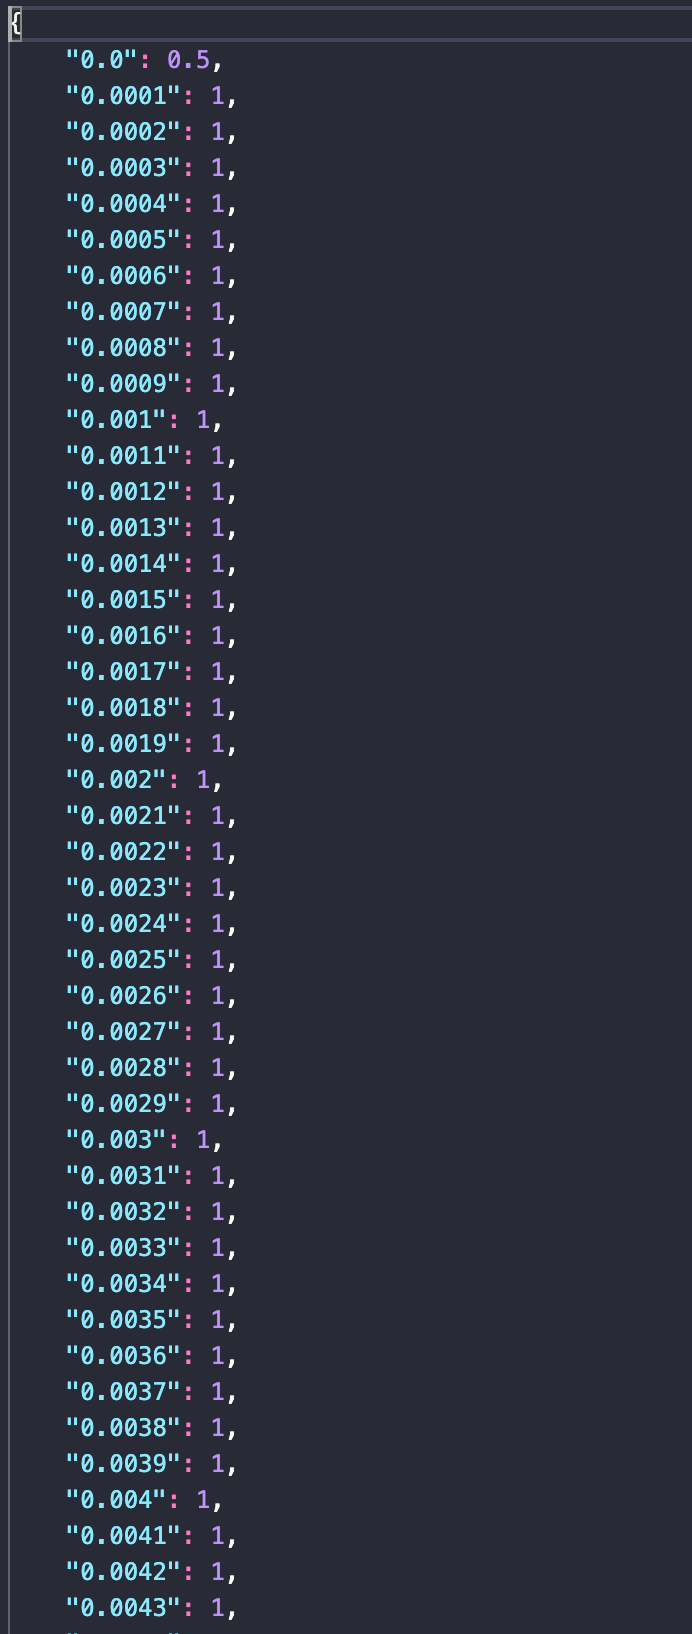
\includegraphics[width=0.38\textwidth]{UncompressedData}
	\end{center}
	\caption{A sample of an uncompressed word storage file}
	\label{fig:uncomp}
\end{wrapfigure}

Figure \ref{fig:uncomp} shows a sample of the representation of the data stored without compression whilst figure \ref{fig:compression} shows the same data after compression. Due to the way the KD signal is generated, there are a large amount of duplicate values. My compression algorithm works by storing the range in values at which the KD signal is the same. In figure \ref{fig:compression} you can quiet clearly see that between the timestamps of 1.5649 and 1.6368 the value did not change from 1. Previously all of the timestamps between these two values would have been stored leading to a bloated file size that contained a lot of unnecessary information.

This type of compression makes a huge impact on the file sizes. For example, the file storing the data in figure \ref{fig:uncomp} without compression is approximately 91 kilobytes whilst the compressed version shown in \ref{fig:compression} is approximately 735 bytes. This is a large saving in terms of space, with the compressed version being 99\% smaller than the compressed version. Whilst 91 kilobytes may not seem like a lot, when the average office worker types at approximately 30 words per minute\cite{naskar_2020} for approximately 8 hours a day leading to around 14400 words typed per day. If even a small percentage such as 10\% of these words are unique, then the resulting uncompressed word data would take up 131040 kilobytes or 131.4 megabytes worth of space. However, if the data is compressed then the same amount of words would only take up 1.05 megabytes. In this particular case this results in savings of 130 megabytes which is a huge amount.

\begin{figure}[h!]
	\begin{lstlisting}
[
    {"key": [1.5647, 1.5647], "value": 0.0}, 
    {"key": [1.5648, 1.5648], "value": 0.5}, 
    {"key": [1.5649, 1.6368], "value": 1.0}, 
    {"key": [1.6369, 1.6369], "value": 0.5},
    {"key": [1.637, 1.664], "value": 0.0}, 
    {"key": [1.6641, 1.6641], "value": 0.5}, 
    {"key": [1.6642, 1.772], "value": 1.0}, 
    {"key": [1.7721, 1.7721], "value": 0.5}, 
    {"key": [1.7722, 1.7955], "value": 0.0}, 
    {"key": [1.7956, 1.7956], "value": 0.5}, 
    {"key": [1.7957, 1.865], "value": 1.0},
    {"key": [1.8651, 1.8651], "value": 0.5}, 
    {"key": [1.8652, 1.9731], "value": 0.0}, 
    {"key": [1.9732, 1.9732], "value": 0.5}, 
    {"key": [1.9733, 2.0206], "value": 1.0}, 
    {"key": [2.0207, 2.0207], "value": 0.5}, 
    {"key": [2.0208, 2.1287], "value": 0.0}, 
    {"key": [2.1288, 2.1288], "value": 0.5}, 
    {"key": [2.1289, 2.2002], "value": 1.0}
]
	\end{lstlisting}
	\caption{KD representation of a user typing hello after compression}
	\label{fig:compression}
\end{figure}



\begin{itemize}
	\item Compression - file sizes too large
	\item Keyboard storage info
\end{itemize}
\section{Pausing}
\begin{itemize}
	\item Uses auth method
	\item why? Sensitive info
	\item Implementation processes??
\end{itemize}
\chapter{Results and Discussion}
\begin{itemize}
	\item Test Results
	\item Calc and use FP, FN, TP, TN - get a percentage
	\item Discuss in relation to validation measure
	\item Mention struggling with small words maybe???
	\item Speed, security??
\end{itemize}
\chapter{Critical Appraisal}
\begin{enumerate}
	\item Summary and crit analysis
	\begin{itemize}
		\item System works very well - provide examples using test data??
		\item System is lightweight and secure
		\item Compared to og planned, system is more complicated
		\item Struggles with smaller words - less data points
		\item NEED TO COME BACK TO THIS, NOT DETAILED AT ALL
	\end{itemize}
	\item Impact
	\begin{itemize}
		\item Benefits 
		\begin{itemize}
			\item better security in combo with other sec methods
			\item Lightweight and users won't notice
			\item Doesn't spy on people due to only storing KDS and can turn off when user is doing something sensitive
			\item Can be adapted to be used in the real word easily
		\end{itemize}
		\item Risks
		\begin{itemize}
			\item Greater surveillance
			\item Could easily be adapted maliciously - key logger
			\item NEED MORE
		\end{itemize}
	\end{itemize}
	\item Personal Development
	\begin{itemize}
		\item Maths, maths, maths
		\item Further git knowledge???
		\item Exp Project Development
		\item MORE
	\end{itemize}
\end{enumerate}
\chapter{Conclusion}
\bibliographystyle{plain}
\bibliography{reference}
\chapter*{Appendix A}

This appendix contains the test data used in figure \ref{fig:WordsvsTime} and the raw data in a table format for this test.

\section*{The Test Paragraph}
The data consisted of a user typing the following paragraph. The paragraph consists of differing lengths and multiple forms of capitalisation and punctuation.

"Hello my name is Jack, I like to do lots of work and play counter strike. I am from Waterbeach although I am going to be living in Landbeach soon. This will be fun with my friend Alex and will ensure that I can relax and continue to work for Ben. I am looking forward to it."

\section*{Results in Table Form}
The results in table form are here. As you can quite clearly see the time increased linearly. The speed of this is impacted by the speed of the computer it is running on. A faster computer will mean that the results are significantly faster.

\begin{center}
	\begin{tabular}{|c|c|}
		Number of Words Chosen & Time \\
	\end{tabular}
\end{center}

\section*{Code Used}
The code used to do this is below. It consists of me using running the validation method with different amounts of words chosen each time until we reach the max number of words chosen.

The code here is very simple and makes use of the rest of my source code. The timeit function\cite{pythonsoftwarefoundation_2022} is part of the default python installation provides a useful function that allows me to accurately time how long functions take. 

\begin{figure}[h!]
	\begin{lstlisting}
		times = {}
		# The typing data is loaded in from a file
		file = open("data.pickle", 'wb')
		data = pickle.load(file) # And then unpacked
		start = 1649857380.5629547 # The start time of when the data was collected in epoch time
		prof = pf.User_Profile() # The user profile used
		presave = t.Training(data, start, prof, 1,0) # Saving all word files immediately
		
		interval = i.Calculation(data, start, prof, 1)
		for x in range(2, interval.noWords, 2):
			print(x)
			interval.chosenAmount = x
			interval.chosen = interval.choose()
			start = timeit.default_timer()
			_, _ = interval.validation(mode='rnl') # Test mode, ensures the pc does not lock or update the data
			times[x] = timeit.default_timer() - start
	\end{lstlisting}
	\caption{Word Selection Testing}
	\label{fig:selTest}
\end{figure}

The data stored in the times dictionary is then plotted with the keys plotted against the values.

\chapter*{Appendix B}

This contains details regarding the validation procedure.

\section*{First Validation Proc Flowchart}

\begin{figure}
	\centering
	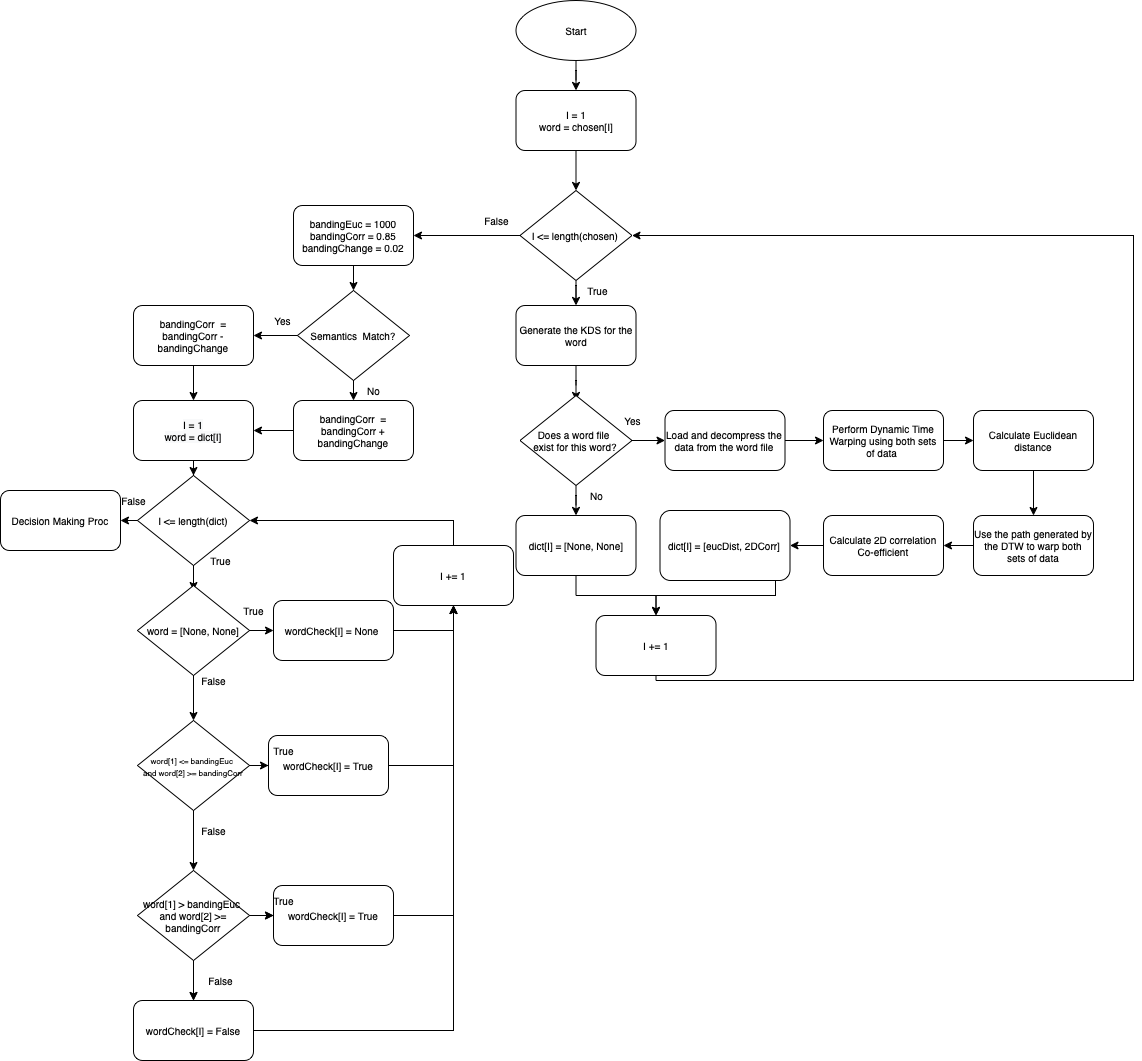
\includegraphics[scale=0.30]{ValidationProc}
	\caption{FLowchart of first element of validation procedure.}
	\label{fig:valProc}
\end{figure}


\end{document}
